\chapter{Techniques for Project Evaluation}
\section{Introduction to Capital and Interest}
\subsection{Capital}
\begin{itemize}
  \item \textbf{Capital} is wealth in the form of money or property that can be used to produce more wealth
  \item A pound is worth more than a pound one or two years from now because of the \textbf{interest} it can earn
  \item Therefore money has a \textbf{time value}
  \item Often the riskiest thing a person can do with money is nothing
\end{itemize}
\subsection{Interest}
\begin{itemize}
  \item Interest pays the providers of capital for:
        \begin{itemize}
          \item Forgoing its use during the time the capital is being used
          \item The risk the investor takes in permitting another person or organisation to use their capital
        \end{itemize}
  \item Investors must decide whether the return on their capital is sufficient to buy into a proposed project or venture
  \item The interest available from an alternative investment is the opportunity cost of using capital in the proposed undertaking
\end{itemize}
\section{Simple interest}
Interest earned or charged that is linearly proportional to the initial amount of the loan (principal), the interest rate, and the number of interest periods for which the principal is committed. Simple interest is not used frequently in modern commercial practice.
\begin{gather}
  I = PNi
\end{gather}
where:
\begin{itemize}
  \item $I$ is total simple interest
  \item $P$ is principal amount lent or borrowed
  \item $N$ is number of interest periods
  \item $i$ is interest rate per interest period
\end{itemize}
The total amount repaid at the end of $N$ interest periods is $P+I$. If \pounds 1000 were loaned for three years at a simple interest rate of 10\% per year, the interest earned would be \pounds 300. The total amount owed at the end of three years would be \pounds 1300.
\section{Compound interest}
Interest earned or charged that is based on the remaining principal amount plus any accumulated interest charges up to the beginning of that period. Compound interest considers the time value of money, and is much more common than simple interest.
\begin{gather}
  I = P\left(1 + i\right)^N - P
\end{gather}
The total amount repaid at the end of $N$ interest periods is $P+I$. If \pounds 1000 were loaned for three years at a compound interest rate of 10\% per year, the interest earned would be \pounds 331. The total amount owed at the end of three years would be \pounds 1331.
\subsection{Compound vs simple interest}
Assume that \pounds 1000 were loaned for three years at an interest rate of 10\% per year.
\begin{figure}[H]
  \centering
  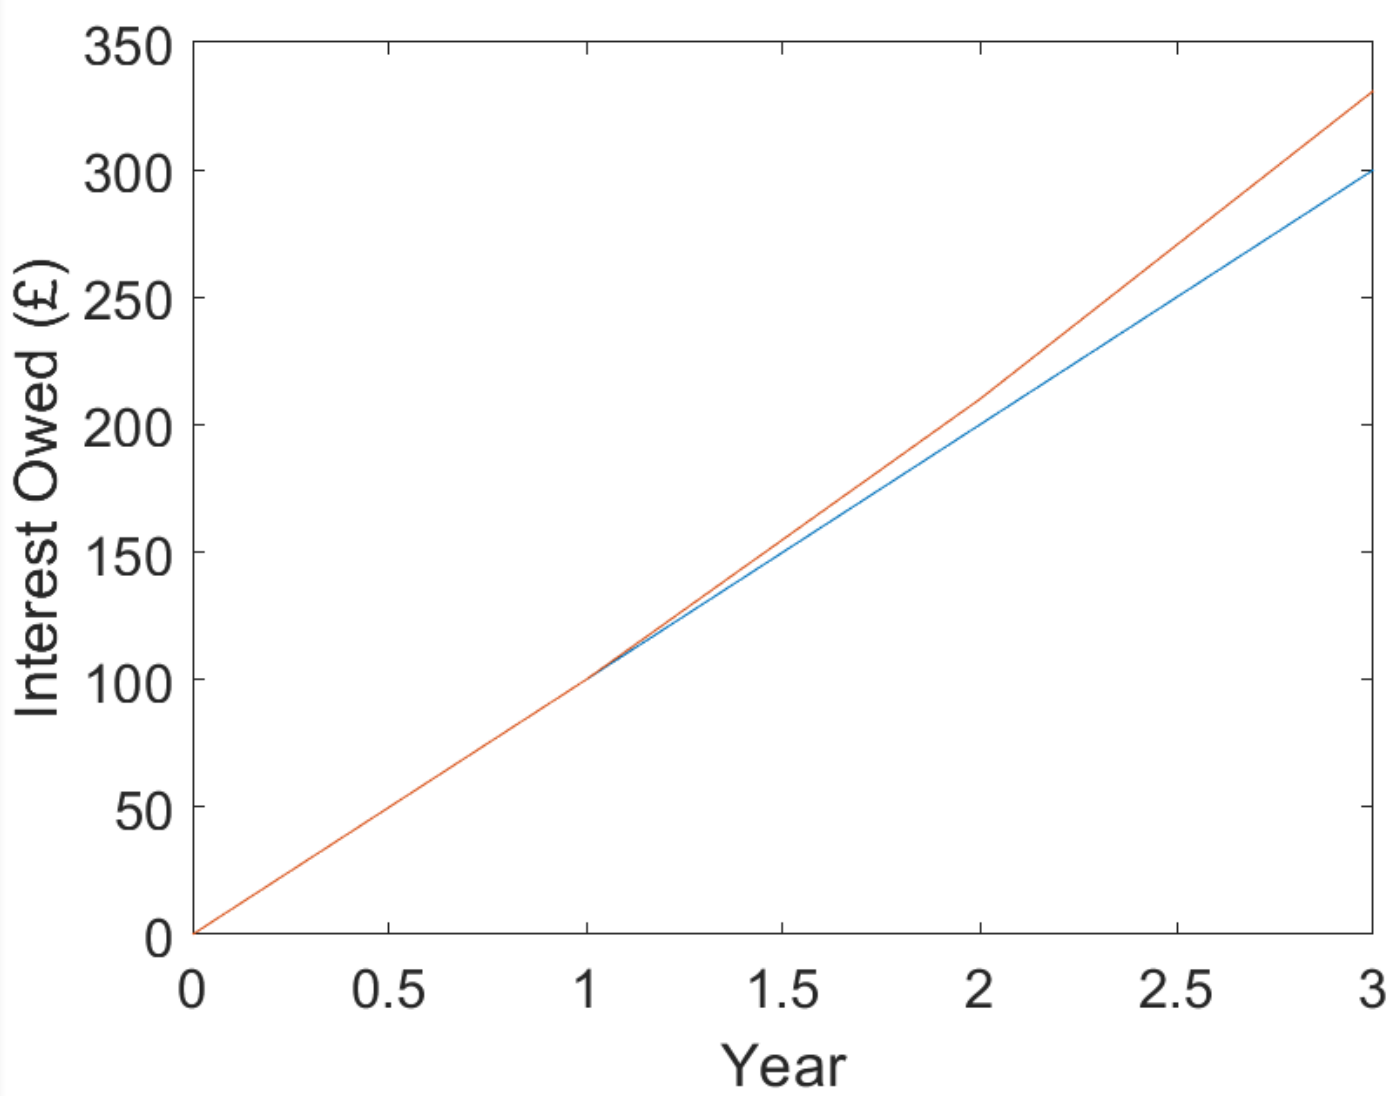
\includegraphics[width = 0.8\textwidth]{./img/figure21.png}
  \caption{Blue: simple interest, Orange: compound interest}
\end{figure}
\section{What is project evaluation}
\begin{itemize}
  \item Project evaluation considers the return that a given project will or should produce
  \item Project evaluation involves quantifying project profitability using various methods
  \item We address whether a proposed capital investment and its associated expenditures can be recovered by revenue (or savings) over a period of time, in addition to a return on the capital that is sufficiently attractive
\end{itemize}
\section{Minimum attractive rate of return (MARR)}
MARR is the \textbf{minimum rate of return} on a project that the top management of an organisation is willing to accept before starting a project. MARR depends on numerous factors:
\begin{itemize}
  \item Amount of money available for investment (as well as the source and costs of funds)
  \item The number of projects available for investment and their purpose (i.e. whether they are essential or optional)
  \item The amount of perceived risk and the estimated cost of administering projects over different planning horizons
  \item The type of organisation involved (government, public utility, private industry)
\end{itemize}
\section{Project evaluation using Net Present Value}
\subsection{Net present value (NPV)}
The NPV method examines the equivalent worth of all cash flows relative to some base point in time i.e. the present. The future value ($FV$) of a sum of money has a value today called the present value ($PV$), which depends on the interest rate / that can be obtained (generally the MARR) - note that we are talking about a single sum of money in this case. The $PV$ of a cashflow in $n$ years' time as a function of $i$ is:
\begin{gather}
  PV = \frac{FV}{\left(1 + i\right)^n}
\end{gather}
Note that $i$ is expressed as a decimal here. A series of uniform (annual) receipts ($AV$) have a value today called the present value ($PV$) which depends on the interest rate / that can be obtained (generally the MARR) - note that we are talking about multiple sums of money in this case. The $PV$ of a series of cashflows that occur at the end of periods (years) 1 to $n$ is:
\begin{gather}
  PV = AV \frac{\left(1+i\right)^n -1}{i\left(1+i\right)^n} = \sum^n_{k=1}\frac{AV}{\left(1+i\right)^k}
\end{gather}
$NPV$ then accounts for all cash inflows and outflows:
\begin{gather}
  NPV = PV_{\textrm{cash inflows}} - PV_{\textrm{cash  outflows}}
\end{gather}
To use the NPV method to determine project worthiness, we compute $NPV$ using the MARR as the interest rate. The higher the interest rate ($i$) and the farther into the future a cash flow occurs, the lower its $PV$.
\begin{figure}[H]
  \centering
  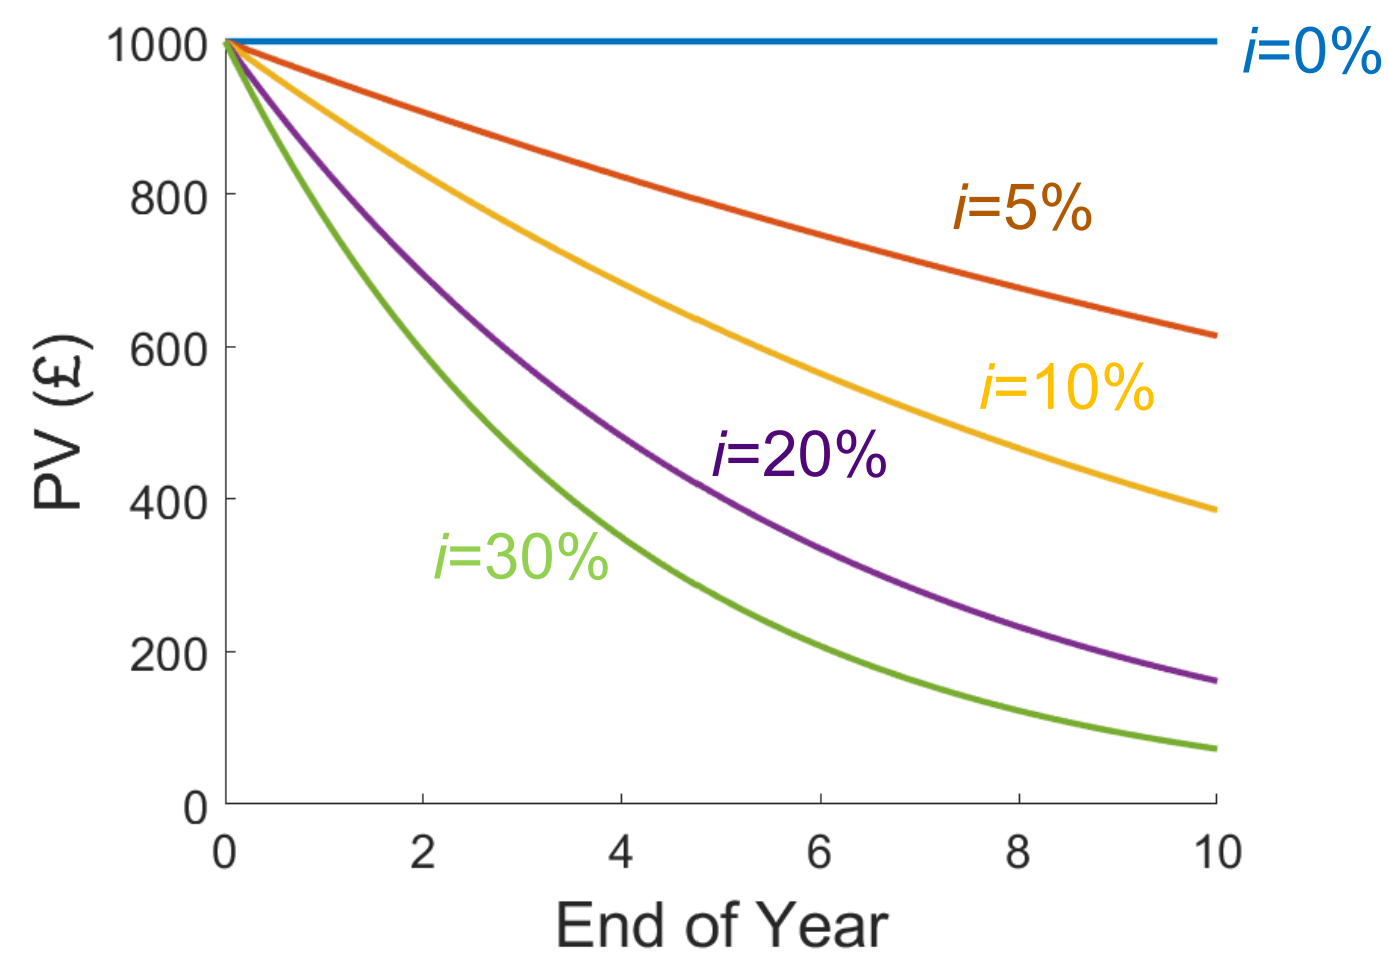
\includegraphics[width = 0.8\textwidth]{./img/figure22.png}
  \caption{Effect of interest rate on PV.}
\end{figure}
\subsection{Example}
A retrofitted heat-pump system is being considered for a small office building. The system can be installed and purchased for \pounds 110,000 and it will save an estimated 300,000 kilowatt-hours of electric power each year over a six-year period. A kilowatt-hour of electricity costs \pounds 0.10, and the company uses a MARR of 15\% per year in its economic evaluations of refurbished systems. The market value of the system will be \pounds 8,000 at the end of six years, and additional annual operating and maintenance expenses are negligible. Use the NPV method to determine whether the system should be installed.
\begin{gather}
  NPV = PV\textrm{ of estimated savings} + PV\textrm{ of market value} -PV\textrm{ of cost}
\end{gather}
Estimated value:
\begin{gather}
  PV_{ES} = 300000\times 0.1 = 30000\\
  PV_{ES,y1} = \frac{30000}{(1+0.15)^1}\\
  PV_{ES,y2} = \frac{30000}{(1+0.15)^2}\dots\\
  PV_{ES,y6} = \frac{30000}{(1+0.15)^6} \\
  \therefore\sum_{k=1}^6\frac{30000}{(1+0.15)^k}
\end{gather}
Market value:
\begin{gather}
  PV_{MV} = \frac{8000}{(1+0.15)^6}
\end{gather}
Cost:
\begin{gather}
  PV_{cost} = 110000
\end{gather}
Therefore, NPV is:
\begin{gather}
  NPV = \sum_{k=1}^6\frac{30000}{(1+0.15)^k} +\frac{8000}{(1+0.15)^6} - 110000 \approx 6993
\end{gather}
\subsection{Advantages and disadvantages of NPV}
Advantages
\begin{itemize}
  \item It accounts for the time value of money
  \item It accounts for uncertainties about future projections
  \item It accounts for all cash flows of interest
\end{itemize}
Disadvantages
\begin{itemize}
  \item It is highly sensitive to the interest rate used
  \item It is not useful for comparing projects of different sizes
  \item It ignores costs that are incurred before the project starts
\end{itemize}
\section{Project evaluation using Internal Rate of Return}
\subsection{Internal Rate of Return (IRR)}
The IRR method solves for the interest rate that equates the present value of cash inflows (receipts or savings) to the present value of cash outflows (expenditures, e.g. investment costs). That is, the IRR provides the answer to the question: what interest rate provides an NPV of 0? This method is the most widely using rate-of-return method for performing engineering economic analyses.
\begin{figure}[H]
  \centering
  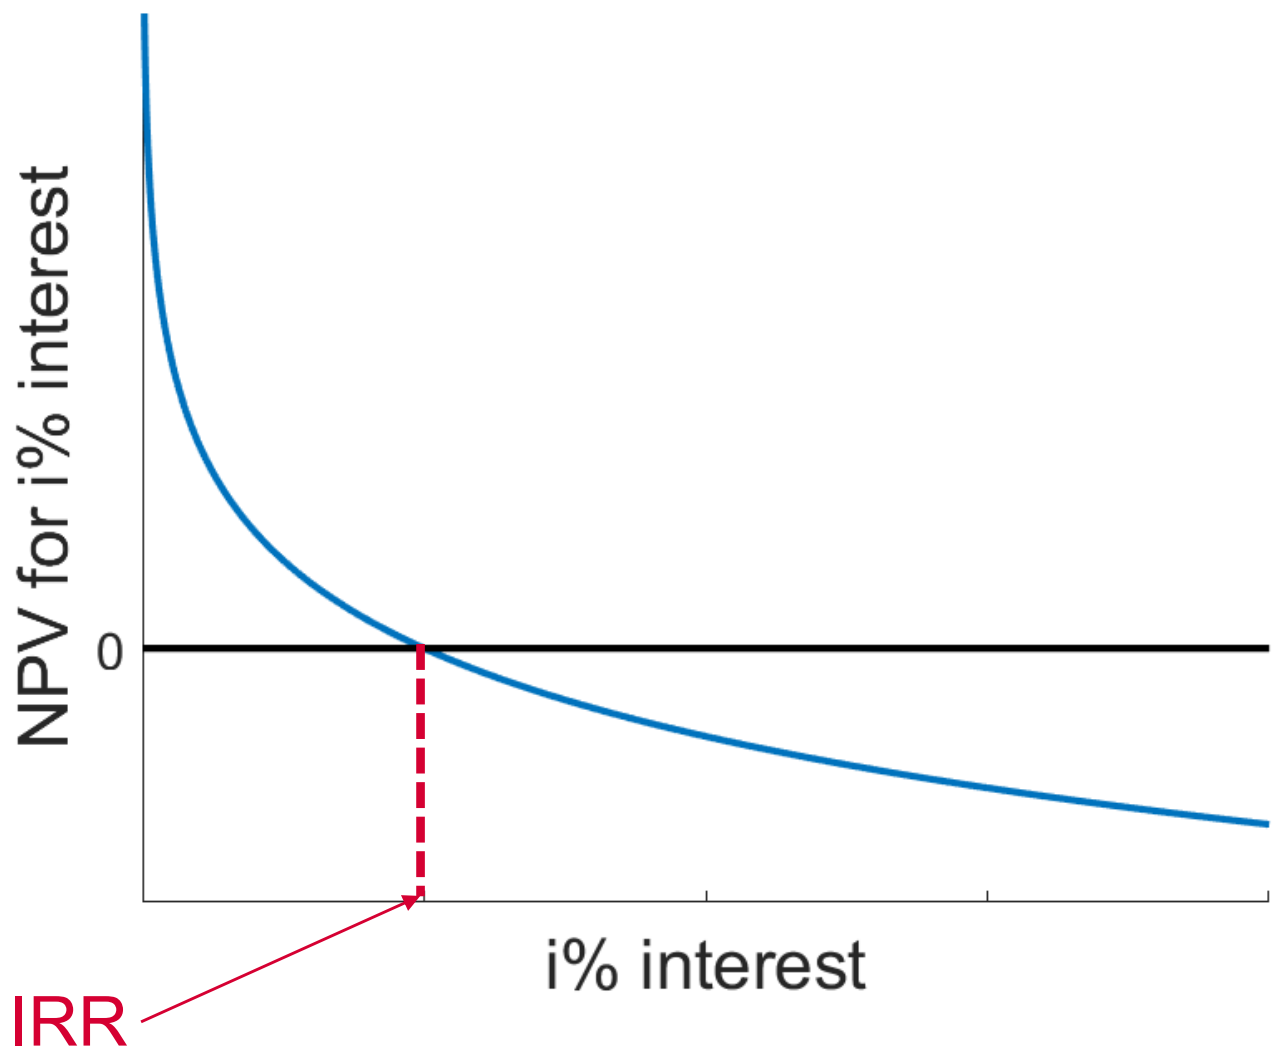
\includegraphics[width = 0.7\textwidth]{./img/figure23.png}
  \caption{Internal Rate of Return.}
\end{figure}
\subsection{Example}
A company is considering the purchase of a digital camera for the maintenance of design specifications by feeding digital pictures directly into an engineering workstation where computer-aided design files can be superimposed over the digital pictures. Differences between the two images can be noted, and corrections as appropriate can then be made by design engineers. The capital investment requirement is \pounds 345,000 and the estimated market value of the system after a six-year study period is \pounds 115,000. Annual revenues attributable to the new system will be \pounds 120,000 and additional annual expenses will be \pounds 22,000. You have been asked by management to determine the IRR of this project and to make a recommendation. The corporation's MARR is 20\% per year.

Denote IRR as $i$. First let's determine an equation for NPV:
\begin{gather}
  NPV = PV \textrm{ of net annual revenue} + PV \textrm{ of market value} - PV \textrm{ of cost}
\end{gather}
PV of net annual revenue:
\begin{gather}
  PV_{NAR,y1} = \frac{120000-22000}{(1+i)^1}\\
  PV_{NAR,y2} = \frac{120000-22000}{(1+i)^2}\dots\\
  PV_{NAR,y6} = \frac{120000-22000}{(1+i)^6}\\
  \therefore \sum_{k=1}^6 \frac{98000}{(1+i)^k}
\end{gather}
Market Value:
\begin{gather}
  PV_{MV} = \frac{115000}{(1+i)^6}
\end{gather}
Cost:
\begin{gather}
  PV_{cost} = 345000
\end{gather}
NPV:
\begin{gather}
  NPV = \sum_{k=1}^6 \frac{98000}{(1+i)^k} + \frac{115000}{(1+i)^6} - 345000
\end{gather}
Lets try $i = MARR = 20\% = 0.2$:
\begin{gather}
  NPV(i=0.2) = + 19,413
\end{gather}
However, this is not the IRR\dots We must calculate $i$ using a solver to find which value of $i$ gives and NPV of 0. Using Excel, we find that our IRR is 22\%. Interpolation may also be used.
\subsection{Advantages and disadvantages of IRR}
Advantages:
\begin{itemize}
  \item It has widespread acceptance in industry
  \item It is relatively simple to understand
  \item It accounts for the time value of money
\end{itemize}
Disadvantages
\begin{itemize}
  \item It is difficult to compute
  \item It ignores the size and scope of projects
  \item It does not account for the actual reinvestment rate
\end{itemize}
\section{Project evaluation using Payback Period}
The payback period method evaluates the number of years $\Theta$ it takes for cash inflows to equal cash outflows. Both of the previous evaluation methods focus on profitability. The payback period instead estimates a company's liquidity (i.e. how fast an investment can be recovered). There are two types of payback period methods:
\begin{enumerate}
  \item Simple payback period - ignores the time value of money
  \item Discounted payback period - accounts for the time value of money
\end{enumerate}
\subsection{Simple Payback Period Example}
A public school is being renovated for \pounds 13.5 million. The building has geothermal heating and cooling, high-efficiency windows, and a solar array that permits the school to sell electricity back to the local electric utility. The annual value of these benefits is estimated to be \pounds 2.7 million. In addition, the residual value of the school at the end of its 40-year life is negligible. What is the simple payback period for the renovated school?

The simple payback period is:
\begin{gather}
  SPP = \frac{13.5}{2.7} = 5 \textrm{ years}
\end{gather}
\subsection{Simple \& Discounted Payback Period Example}
A piece of new equipment has been proposed by engineers to increase the productivity of a certain manual welding operation. The investment cost is \pounds 25,000 and the equipment will have a market value of \pounds 5,000 at the end of its expected life of 5 years. Increased productivity attributable to the equipment will amount to \pounds 8,000 per year after extra operating costs have been subtracted from the value of the additional production. MARR is 20\% per year. Calculate the simple and the discounted payback periods.
\begin{figure}[H]
  \centering
  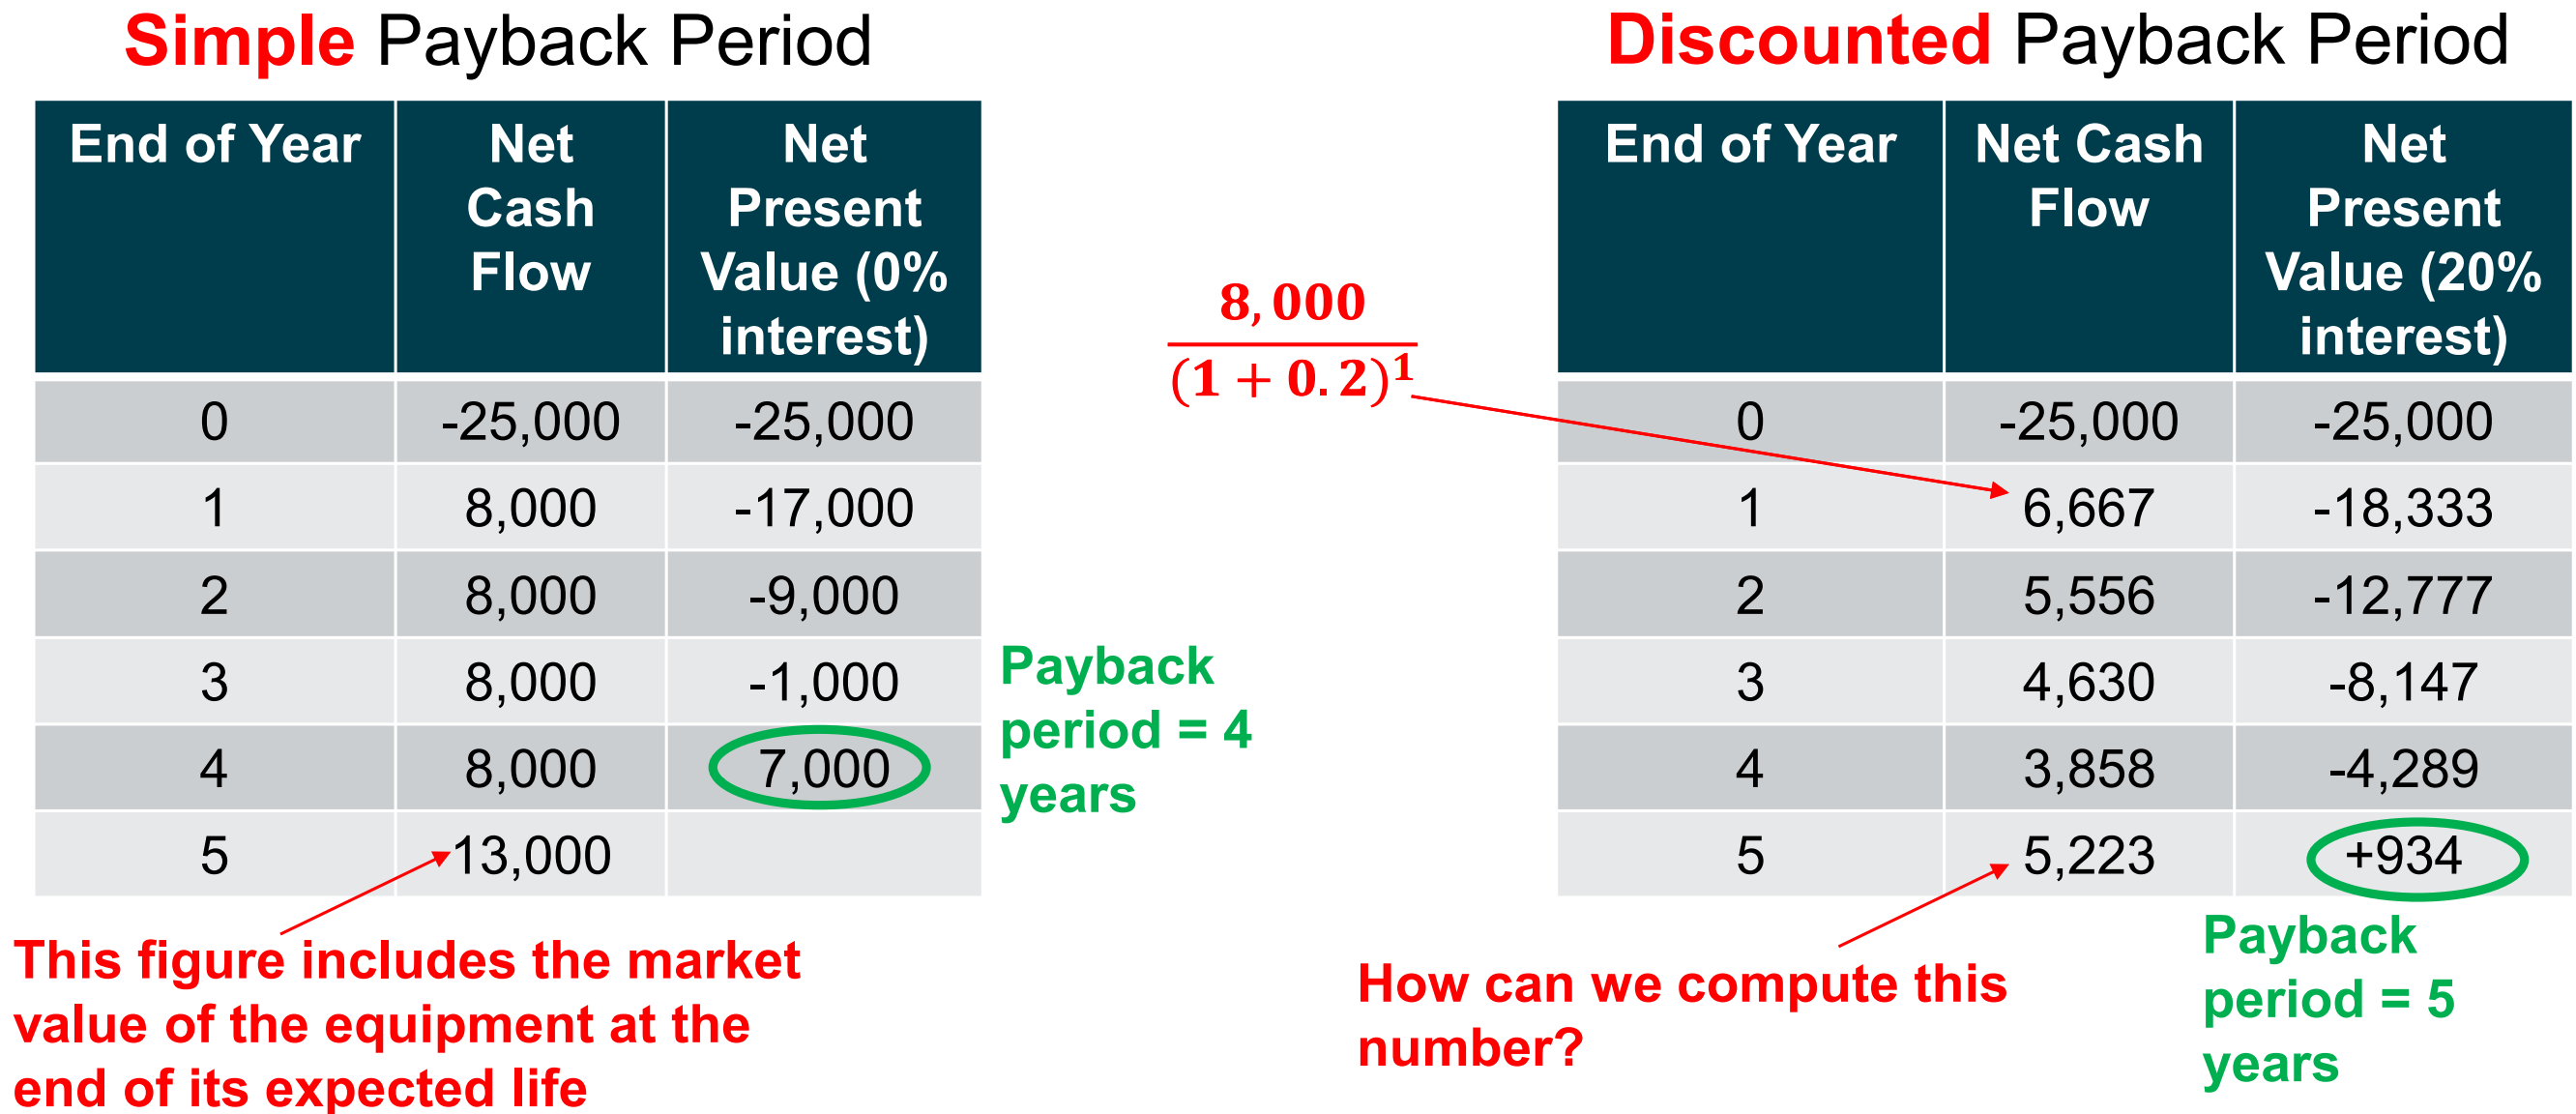
\includegraphics[width = \textwidth]{./img/figure24.png}
  \caption{Simple and discounted payback periods.}
\end{figure}
\subsection{Advantages and disadvantages of payback period}
Advantages
\begin{itemize}
  \item It provides a new perspective on performance (by focusing on liquidity)
  \item It is relatively simple to understand and compute
  \item It requires relatively few inputs
\end{itemize}
Disadvantages
\begin{itemize}
  \item It does not account for cash flows that occur after the payback period
  \item It may not consider the time value of money
  \item It ignores profitability, and should only be used as a secondary evaluation measure.
\end{itemize}